%!TEX root = /Users/louis/Documents/PhD/Deliverables/Thesis/thesis.tex

\section{Textual Modelling Notation}
\label{sec:notation}
The analysis of co-evolution examples in Chapter~\ref{Analysis} highlighted two ways in which co-evolution is managed. In \emph{developer-driven} co-evolution, migration is specified by the metamodel developer in an executable format; while in \emph{user-driven co-evolution} migration is specified by the metamodel developer in prose or not at all. Performing user-driven co-evolution with modelling frameworks presents two key challenges that have not been explored by existing research. Firstly, user-driven co-evolution frequently involves editing the storage representation of the model, such as XMI. Model storage representations are typically not optimised for human use and hence user-driven co-evolution can be error-prone. Secondly, non-conformant model elements must be identified during user-driven co-evolution. When a multi-pass parser is used to load models, as is the case with EMF, not all conformance problems are reported at once, and user-driven co-evolution is an iterative process. In Section~\ref{sec:requirements_identification}, these challenges lead to the identification of the following requirement: \emph{This thesis must demonstrate a user-driven co-evolution process that enables the editing of non-conformant models without directly manipulating the underlying storage representation and provides a sound and complete conformance report for the original model and evolved metamodel.}

The remainder of this section describes a textual notation for models, which has been implemented for EMF, and discusses the way in which the notation has been integrated with the metamodel independent syntax described in Section~\ref{sec:mmi_syntax} to produce conformance reports. 


\subsection{Human-Usable Textual Notation}
\label{subsec:hutn}
The OMG's Human-Usable Textual Notation (HUTN) \cite{hutn} defines a textual modelling notation, which aims to conform to human-usability criteria \cite{hutn}. There is no current reference implementation of HUTN: the Distributed Systems Technology Centre's TokTok project (an implementation of the HUTN specification) is inactive (and the source code can no longer be found), whilst implementation of HUTN described in \cite{muller05hutn} has been abandoned in favour of Sintaks\footnote{\url{http://www.kermeta.org/sintaks/}}, which operates on domain-specific concrete syntax.

Model storage representations are often optimised for reducing storage space or increasing the speed of random access, rather than for human usability. By contrast, the HUTN specification states its primary design goal as human-usability and ``this is achieved through consideration of the successes and failures of common programming languages'' \cite[Section 2.2]{hutn}. The HUTN specification refers to two studies of programming language usability to justify design decisions, but, because no reference implementation exists, the specification does not evaluate the human-usability of the notation. As HUTN is optimised for human-usability, using HUTN rather than XMI for user-driven co-evolution might lead to increased developer productivity. This claim is explored in Chapter~\ref{Evaluation}.

Like the generic metamodel presented in Section~\ref{sec:mmi_syntax}, HUTN is a metamodel-independent syntax for 
MOF. However, the HUTN specification focuses on concrete syntax, whereas the metamodel-independent syntax presented in Section~\ref{sec:mmi_syntax} focuses on abstract syntax. In this section, the key features of HUTN are introduced, and the sequel introduces a reference implementation of HUTN. To illustrate the notation, the MOF-based metamodel of families in Figure \ref{fig:example-mm} is used. The \texttt{nu\-cl\-e\-ar} attribute on the \texttt{Fa\-mi\-ly} class is used to indicate that the family ``comprises only a father, a mother, and children.'' \cite{nucleardef}.

\begin{figure}[htbp]
  \begin{center}
    \leavevmode
    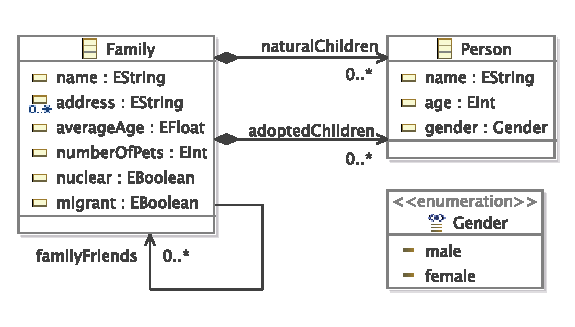
\includegraphics[scale=0.85]{5.Implementation/images/families.pdf}
  \end{center}
  \caption{Exemplar families metamodel}
  \label{fig:example-mm}
\end{figure}


\subsubsection{Basic Notation}
Listing \ref{lst:attributes} shows the construction of an \emph{object} in HUTN, here an instance of the Family class from Figure \ref{fig:example-mm}. Line 1 specifies the package containing the classes to be constructed (\texttt{FamilyPackage}) and a corresponding identifier (\texttt{families}), used in fully-qualified references to objects (Section \ref{subsubsec:inter-package_references}). Line 2 names the class (\texttt{Family}) and gives an identifier for the object (\texttt{The Smiths}). Lines 3 to 7 define \emph{attribute values}; in each case, the data value is assigned to the attribute with the specified name. The encoding of the value depends on its type: strings are delimited by any form of quotation mark; multi-valued attributes use comma separators, etc.

The metamodel in Figure \ref{fig:example-mm} defines a \emph{simple reference} (familyFriends) and two \emph{containment references} (adoptedChildren; naturalChildren). The HUTN representation embeds a contained object directly in the parent object, as shown in Listing \ref{lst:containment}. A simple reference can be specified using the type and identifier of the referred object, as shown in Listing \ref{lst:non-contained}. Like attribute values, both styles of reference are preceded by the name of the meta-feature.

\begin{lstlisting}[caption=Specifying attributes with HUTN., label=lst:attributes, language=HutnFamilies]
FamilyPackage "families" {
    Family "The Smiths" {
        nuclear: true
        name: "The Smiths"
        averageAge: 25.7
        numberOfPets: 2
        address: "120 Main Street", "37 University Road"
    }
}
\end{lstlisting}

\begin{lstlisting}[caption=Instantiation of naturalChildren -- a HUTN containment reference., label=lst:containment, language=HutnFamilies]
FamilyPackage "families" {
    Family "The Smiths" {
        naturalChildren: Person "John" { name: "John" },
                                Person "Jo" { gender: female }
    }
}
\end{lstlisting}


\begin{lstlisting}[caption=Specifying a simple reference with HUTN., label=lst:non-contained, language=HutnFamilies]
FamilyPackage "families" {
    Family "The Smiths" {
        familyFriends: Family "The Does"
    }
    Family "The Does" {}
}
\end{lstlisting}


\subsubsection{Keywords and Adjectives}
While HUTN is unlikely to be as concise as a metamodel-specific concrete syntax, the notation does define syntactic shortcuts to make model specifications more compact. Shortcut use is optional, and the HUTN specification aims to make their syntax intuitive \cite[pg2-4]{hutn}. Two example notational shortcuts are described here, to illustrate some of the ways in which HUTN can be used to construct models in a concise manner.

When specifying a \emph{Boolean-valued attribute}, it is sufficient to simply use the attribute name (value \texttt{true}), or the attribute name prefixed with a tilde (value \texttt{false}). When used in the body of the object, this style of Boolean-valued attribute represents a \emph{keyword}. A keyword used to prefix an object declaration is called an \emph{adjective}. Listing \ref{lst:boolean} shows the use of both an attribute keyword (\texttt{\textasciitilde nuclear} on line 6) and adjective (\texttt{\textasciitilde migrant} on line 2).

\begin{lstlisting}[caption=Using keywords and adjectives in HUTN., label=lst:boolean, language=HutnFamilies]
FamilyPackage "families" {
    ~migrant Family "The Smiths" {}

    Family "The Does" {
        averageAge: 20.1
        ~nuclear
        name: "The Does"
    }
}
\end{lstlisting}


\subsubsection{Inter-Package References}
\label{subsubsec:inter-package_references}
To conclude the summary of the notation, two advanced features defined in the HUTN specification are discussed. The first enables objects to refer to other objects in a different package, while the second provides means for specifying the values of a reference for all objects in a single construct (which can be used, in some cases, to simplify the specification of complicated relationships).

\begin{lstlisting}[caption=Referencing objects in other packages with HUTN., label=lst:fullyqualified, language=HutnFamilies]
FamilyPackage "families" {
    Family "The Smiths" {}
}
VehiclePackage "vehicles" {
    Vehicle "The Smiths' Car" {
        owner: FamilyPackage.Family "families"."The Smiths"
    }
}
\end{lstlisting}

To reference objects between separate package instances in the same document, the package identifier is used to construct a fully-qualified name. Suppose a second package is introduced to the metamodel in Figure \ref{fig:example-mm}. Among other concepts, this package introduces a Vehicle class, which defines an owner reference of type Family. Listing \ref{lst:fullyqualified} illustrates the way in which the owner feature can be populated. Note that the fully-qualified form of the class utilises the names of elements of the metamodel, while the fully-qualified form of the object utilises only HUTN identifiers defined in the current document.

The HUTN specification defines name scope optimisation rules, which allow the definition above to be simplified to: \texttt{owner: Family "The Smiths"}, assuming that the VehiclePackage does not define a Family class, and that the identifier ``The Smiths'' is not used in the VehiclePackage block.


\subsubsection{Alternative Reference Syntax}
In addition to the syntax defined in Listings \ref{lst:containment} and \ref{lst:non-contained}, the value of references may be specified independently of the object definitions. For example, Listing \ref{lst:assocblock} demonstrates this alternate syntax by defining The Does as friends with both The Smiths and The Bloggs.

\begin{lstlisting}[caption=Using a reference block in HUTN., label=lst:assocblock, language=HutnFamilies]
FamilyPackage "families" {
    Family "The Smiths" {}
    Family "The Does" {}
    Family "The Bloggs" {}
    
    familyFriends {
        "The Does" "The Smiths"
        "The Does" "The Bloggs"
    }
}
\end{lstlisting}

Listing \ref{lst:associnfix} illustrates a further alternative syntax for references, which employs an infix notation. 

\begin{lstlisting}[caption=Using an infix reference in HUTN., label=lst:associnfix, language=HutnFamilies]
FamilyPackage "families" {
    Family "The Smiths" {}
    Family "The Does" {}
    Family "The Bloggs" {}
    
    Family "The Smiths" familyFriends Family "The Does";
    Family "The Smiths" familyFriends Family "The Bloggs";
}
\end{lstlisting}

The reference block (Listing~\ref{lst:assocblock}) and infix (Listing~\ref{lst:associnfix}) notations are syntactic variations on -- and have identical semantics to -- the reference notation shown in Listings \ref{lst:containment} and \ref{lst:non-contained}.


\subsubsection{Customisation via Configuration}
Some limited customisation of HUTN for particular metamodels can be achieved using \emph{configuration files}. Customisations permitted include a parametric form of object instantiation; renaming of metamodel elements; specifying the default value of a feature; and providing a default identifier for classes of object.


\subsection{Epsilon HUTN}
\label{subsec:epsilon_hutn}
To investigate the extent to which HUTN can be used during user-driven co-evolution, an implementation, Epsilon HUTN, was constructed. This section describes the way in which Epsilon HUTN was implemented using a combination of model-management operations. From text conforming to the HUTN syntax (described above), Epsilon HUTN produces an equivalent model that can be managed with the Eclipse Modeling Framework (EMF) \cite{steinberg09emf}. The sequel demonstrates the way in which Epsilon HUTN can be used for user-driven co-evolution.

\subsubsection{Implementation of Epsilon HUTN}
Epsilon HUTN, makes extensive use of the Epsilon model management platform, which was introduced in Section~\ref{subsec:epsilon}. Epsilon provides infrastructure for implementing uniform and interoperable model management languages, for performing tasks such as model merging, model transformation and inter-model consistency checking. Epsilon HUTN is implemented using the model-to-model transformation (ETL), model-to-text transformation (EGL) and model validation (EVL) languages of Epsilon. Although any languages for model-to-model transformation 
(M2M), model-to-text transformation (M2T) and model validation could have been used, Epsilon's existing domain-specific languages are tightly integrated and inter-operable, making it feasible to chain model management operations together to implement Epsilon HUTN.

\begin{figure}[htbp]
  \begin{center}
    \leavevmode
    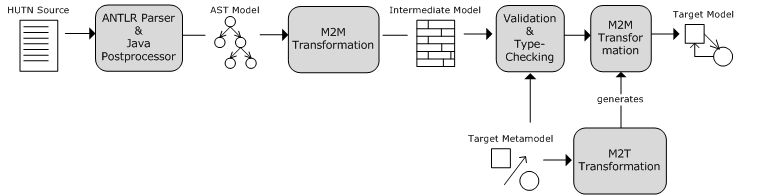
\includegraphics[scale=0.44]{5.Implementation/hutn_workflow.png}
  \end{center}
  \caption{The architecture of Epsilon HUTN.}
  \label{fig:architecture}
\end{figure}

Figure \ref{fig:architecture} outlines the workflow through Epsilon HUTN, from HUTN source text to instantiated target model. The HUTN model specification is parsed to an abstract syntax tree using a HUTN parser specified in ANTLR \cite{parr07antlr}. From this, a Java postprocessor is used to construct an instance of a simple AST metamodel (which comprises two meta-classes, Tree and Node). Using ETL, M2M transformations are then applied to produce an intermediate model, which is an instance of the generic metamodel discussed in Section~\ref{sec:mmi_syntax}. Finally, a M2T transformation on the target metamodel, specified in EGL, produces a further M2M transformation, which consumes the intermediate model and produces the target model.

The workflow uses an extension of the generic metamodel defined in Section~\ref{sec:mmi_syntax}. Because the HUTN specification allows the use of packages, an extra element, \texttt{PackageObject}, was added to the generic metamodel. A \texttt{PackageObject} has a type, an optional identifier and contains any number of \texttt{Object}s. To avoid confusion with \texttt{PackageObjects}, the \texttt{Object} class in the generic metamodel was renamed to \texttt{ClassObject}.

Using two M2M transformation stages with the (extended) generic metamodel as an intermediary has two advantages. Firstly, the form of the AST metamodel is not suited to a one-step transformation. There is a mismatch between the features of the AST metamodel and the needs of the target model -- for example, between the Node class in the AST metamodel and classes in the target metamodel. If a one-step transformation were used, each transformation rule would need a lengthly guard statement, which is hard to understand and verify. Secondly, Section~\ref{sec:mmi_syntax} discussed a mechanism for binding XMI to the generic metamodel, which can be used in conjunction with the latter half of the Epsilon HUTN workflow (Figure~\ref{fig:architecture}) to generate HUTN from XMI. This process is discussed further in Section~\ref{subsec:migration_with_hutn}.

Throughout the remainder of this section, instances of the generic metamodel producing during the execution of the HUTN workflow are termed an \textit{intermediate model}. The two M2M transformations are now discussed in depth, along with a model validation phase which is performed prior to the second transformation.

\paragraph{AST Model to Intermediate Model}
Epsilon HUTN uses ETL \cite{kolovos08etl} for specifying M2M transformation. One of the transformation rules from Epsilon HUTN is shown in Listing \ref{lst:m2m}. The rule transforms a name node in the AST model (which could represent a package or a class object) to a package object in the intermediate model. The guard (line 5) specifies that a name node will only be transformed to a package object if the node has no parent (i.e. it is a top-level node, and hence a package rather than a class). The body of the rule states that the type, line number and column number of the package are determined from the text, line and column attributes of the node object. On line 11, a containment slot is instantiated to hold the children of this package object. The children of the node object are transformed to the intermediate model (using a built-in method, \verb|equivalent()|), and added to the containment slot.

\begin{lstlisting}[caption=Transformation rule (in ETL) to convert AST nodes to package objects., label=lst:m2m, language=ETL]
rule NameNode2PackageObject
    transform n : AntlrAst!NameNode
    to p : Intermediate!PackageObject {

    guard : n.parent.isUndefined()

    p.type := n.text;
    p.line := n.line;
    p.col  := n.column;

    var slot := new Intermediate!ContainmentSlot;
    for (child in n.children) {
        slot.objects.add(child.equivalent());
    }
    if (slot.objects.notEmpty()) {
        p.slots.add(slot);
    }
}
\end{lstlisting}

\paragraph{Intermediate Model Validation}
An advantage of the two-stage transformation is that contextual analysis can be specified in an abstract manner -- that is, without having to express the traversal of the AST. This gives clarity and minimises the amount of code required to define syntatic constraints.

\begin{lstlisting}[caption=A constraint (in EVL) to check that all identifiers are unique., label=lst:constraint, language=EVL]
context ClassObject {
    constraint IdentifiersMustBeUnique {
        guard: self.id.isDefined()
        check: ClassObject.all
                   .select(c|c.id = self.id).size() = 1;
        message: `Duplicate identifier: ' + self.id
    }
}
\end{lstlisting}

Epsilon HUTN uses EVL \cite{kolovos08evl} to specify verification, resulting in highly expressive syntactic constraints. An EVL constraint comprises a guard, the logic that specifies the constraint, and a message to be displayed if the constraint is not met. For example, Listing \ref{lst:constraint} specifies the constraint that every HUTN class object has a unique identifier.

In addition to the syntactic constraints defined in the HUTN specification, the conformance constraints described in Section~\ref{sec:mmi_syntax} are also specified in EVL and are also executed on the model at this stage.

\paragraph{Intermediate Model to Target Model}
When the intermediate model conforms to the target metamodel, the intermediate model can be transformed to an instance of the target metamodel. In generating the target model from the intermediate model (Figure \ref{fig:architecture}), the transformation uses information from the target metamodel, such as the names of classes and features. A typical approach to this category of problem is to use a higher-order transformation on the target metamodel to generate the desired transformation. Epsilon HUTN uses a different approach: the transformation to the target model is produced by executing a M2T transformation on the target metamodel. EGL \cite{rose08egl} is a template-based M2T language. \verb|[% %]| tag pairs are used to denote dynamic sections, which may produce text when executed. Any code not enclosed in a \verb|[% %]| tag pair is included verbatim in the generated text.

Listing \ref{lst:generate} shows part of the M2T transformation used by HUTN. The M2T transformation generates a M2M transformation which specifies the way in which the intermediate model is transformed to the target model. The loop beginning on line 1 of Listing \ref{lst:generate} iterates over each meta-class in the target metamodel, producing a M2M transformation rule. The generated transformation rule consumes a class objects in the intermediate model and produces an element of the target model. The guard of the generated transformation rule (line 6) ensures that only class objects with a type equal to the current meta-class are transformed by the generated rule. To generate the body of the rule, the M2T transformation iterates over each structural feature of the current meta-class, and generates appropriate transformation code for populating the values of each structural feature from the slots on the class object in the intermediate model. The part of the M2T transformation that generates the body of M2M transformation rule is omitted in Listing~\ref{lst:generate} because it contains a large amount of code for interacting with EMF, which is not relevant to this discussion.

\begin{lstlisting}[caption=Part of the M2T transformation (in EGL) for generating the intermediate model to target model transformation (in ETL)., label=lst:generate, language=EGL]
[% for (class in EClass.allInstances()) { %]
rule Object2[%=class.name%]
  transform o : Intermediate!ClassObject
  to t : Model![%=class.name%] {

    guard: o.type = `[%=class.name%]'

    -- body omitted
  }
[% } %]
\end{lstlisting}

For example, executing the M2T transformation in Listing \ref{lst:generate} on the Families metamodel (Figure~\ref{fig:example-mm}) generates the two M2M transformation rules shown in Listing~\ref{lst:hutn_generated_transformation}. The rules produce instances of Family and Person from instances of ClassObject in the intermediate model. The body of each rule copies the values from the slots of the ClassObject to the Family or Person in the target model. Lines 7-9, for example, copy the value of the name slot (if one is specified) to the target Family.

\begin{lstlisting}[caption=The M2M transformation generated by HUTN for the Families metamodel, label=lst:hutn_generated_transformation, language=ETL]
rule Object2Family
  transform o : Intermediate!ClassObject
  to t : Model!Family {

    guard: o.type = `Family'

    if (o.hasSlot(`name')) {
			t.name := o.findSlot(`name').values.first;
		}
		
		if (o.hasSlot(`address')) {
			for (value in o.findSlot(`address').values) {
				t.address.add(value);
			}
		}
		
		-- remainder of body omitted
  }

rule Object2Person
  transform o : Intermediate!ClassObject
  to t : Model!Person {

    guard: o.type = `Person'

    if (o.hasSlot(`name')) {
			t.name := o.findSlot(`name').values.first;
		}
		
		-- remainder of body omitted
  }
\end{lstlisting}

Presently, Epsilon HUTN can be used only to generate EMF models. Support for other modelling languages would require different transformations between intermediate and target model. In other words, for each target modelling language, a new EGL template would be required. The transformation from AST to intermediate model is independent of the target modelling language and would not need to change.


\subsection{Migration with HUTN}
\label{subsec:migration_with_hutn}
Migrating non-conformant models with HUTN involves transforming the XMI of the non-conformant model to HUTN, reconciling the conformance problems in the HUTN source by hand, and transforming the reconciled HUTN back to XMI. The transformations to and from XMI can be automated, and the way in which Epsilon HUTN transforms from HUTN to XMI was described above. Because Epsilon HUTN uses the metamodel-independent syntax (from Section~\ref{sec:mmi_syntax}) as an intermediary, transformation from XMI to HUTN is implemented as follows: the metamodel-independent syntax is used to parse the XMI and produce an intermediate model. Subsequently, an unparser (implemented using the visitor design pattern \cite{gamma95patterns}) generates HUTN source for each element of the intermediate model. In this manner, HUTN can be generated for any XMI document, regardless of whether the model described by the XMI conforms to its metamodel.

To demonstrate the way in which HUTN can be used to perform migration, the exemplar XMI shown in Listing~\ref{lst:xmi} is represented using HUTN in Listing~\ref{lst:non-conformant_hutn}. Recall that the XMI describes three Persons, Franz, Julie and Hermann. Julie and Hermann are the mother and father of Franz.

\begin{lstlisting}[caption=HUTN for people with mothers and fathers., label=lst:non-conformant_hutn, language=HutnFamilies]
Persons "kafkas" {
    Person "Franz"   { name: "Franz"   }
    Person "Julie"   { name: "Julie"   }
    Person "Hermann" { name: "Hermann" }
    
    Person "Franz" mother Person "Julie";
    Person "Franz" father Person "Hermann";
}
\end{lstlisting}

Note that, by using a configuration file to specify that a Person's name is taken from its identifier, the body of the Person objects could be omitted.

If the Persons metamodel now evolves such that mother and father are merged to form a parents reference, Epsilon HUTN reports conformance problems on the HUTN document, as illustrated by the screenshot in Figure~\ref{fig:hutn_conformance_reporting}.

\begin{figure}[htbp]
  \begin{center}
    \leavevmode
    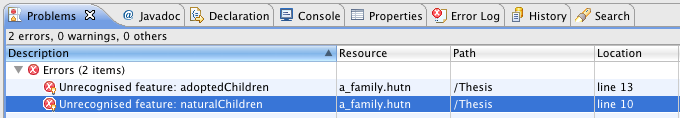
\includegraphics[scale=0.44]{5.Implementation/hutn_conformance_reporting.png}
  \end{center}
  \caption{Conformance problem reporting in Epsilon HUTN.}
  \label{fig:hutn_conformance_reporting}
\end{figure}

Resolving the conformance problems requires the user to change the feature named in the infix associations from mother (father) to parents. The Epsilon HUTN development tools provide content assistance, which might be useful in this situation. Listing~\ref{lst:conformant_hutn} shows a HUTN document that conforms to the metamodel defining parents rather than mother and father.

\begin{lstlisting}[caption=HUTN for people with parents., label=lst:conformant_hutn, language=HutnFamilies]
Persons "kafkas" {
    Person "Franz"   { name: "Franz"   }
    Person "Julie"   { name: "Julie"   }
    Person "Hermann" { name: "Hermann" }
    
    Person "Franz" parents Person "Julie";
    Person "Franz" parents Person "Hermann";
}
\end{lstlisting}


\subsection{Limitations}
During the development of Epsilon HUTN, two primary limitations of the notation became apparent. The first relates to the nature of a metamodel-independent syntax, and the latter to the suitability of HUTN for performing user-driven co-evolution.

\subsubsection{Generic vs specific concrete syntax}
Notwithstanding the power of genericity, there are situations where a metamodel-specific concrete syntax is preferable. An example of where HUTN is unhelpful arose when developing a metamodel for the recording of failure behaviour of components in complex systems, based on the work of \cite{wallace05modular}.

Failure behaviours comprise a number of expressions that specify how each component reacts to system faults, and there is an established concrete syntax for expressing failure behaviours. The failure syntax allows various shortcuts, such as the use of underscore to denote a wildcard. For example, the syntax for a possible failure behaviour of a component that receives input from two other components (on the left-hand side of the expression), and produces output for a single component is denoted:

\begin{eqnarray}\label{failure}
(\{\_\}, \{\_\}) \rightarrow (\{late\})
\end{eqnarray}

The above expression is written using a domain-specific syntax. In HUTN, the specification of these behaviours is less concise. For example, Listing \ref{lst:fptc-hutn} gives the HUTN syntax for failure behaviour (\ref{failure}), above.

\begin{lstlisting}[caption=Failure behaviour specified in HUTN., label=lst:fptc-hutn, language=FPTC]
Behaviour {
    lhs: Tuple {
        contents: IdentifierSet { contents: Wildcard {} },
                     IdentifierSet { contents: Wildcard {} }
    }

    rhs: Tuple {
        contents: IdentifierSet { contents: Fault "late" {} }
    }
}
\end{lstlisting}

The domain-specific syntax exploits two characteristics of failure expressions to achieve a compact notation. Firstly, structural domain concepts are mapped to symbols: tuples to parentheses and identifier sets to braces. Secondly, little syntactic sugar is needed for many domain concepts, as they define only one feature: a fault is referred to only by its name, the contents of identifier sets and tuples are separated using only commas.

In general, HUTN is less concise than a domain-specific syntax for metamodels containing a large number of classes with few attributes, and in cases where most attributes are used to define structural relationships among concepts. However, a domain-specific syntax is specified using metamodel concepts and hence can be affected by metamodel evolution.

\subsubsection{Optimised XMI omits type information}
When HUTN is used for user-driven co-evolution, non-conformant models (represented in XMI) are transformed to HUTN source. The default EMF serialisation mechanism is configure to reduce the size of models on disk and consequently the XMI produced by EMF omits type information when it may be inferred from a metamodel. This is problematic for managing co-evolution because, when a metamodel evolves, type information might be erased. The implementation of Epsilon HUTN has been extended to account for optimised XMI, and reports type inference errors along with conformance problems. 

\subsection{Summary}
In this section, HUTN was introduced and its syntax described. An implementation of HUTN for EMF, built atop Epsilon, was discussed. Integration of HUTN for the metamodel-independent syntax discussed in Section~\ref{sec:mmi_syntax} facilitates user-driven co-evolution with a textual modelling notation other than XMI, as demonstrated by the example above. The remainder of this chapter focuses on developer-driven co-evolution, in which model migration strategies are executable.